\documentclass[10pt]{ujarticle}
\usepackage[top=30truemm, bottom=30truemm, left=25truemm, right=25truemm]{geometry}
\usepackage{listings}
\usepackage{ascmac}
\usepackage{amssymb}
\usepackage{amsmath}
\usepackage{bm}
\usepackage{url}
\usepackage{braket}
\usepackage[dvipdfmx]{hyperref}
\usepackage[dvipdfmx]{graphicx,color}

\title{スピン物性特論レポート}
\author{g1840624 鷲津 優維}
\date{2019/03/29}

\begin{document}
\maketitle
%toi1
\section{スピン流ー熱流変換現象の可視化}
\subsection{現象の概略}
物質中に存在する様々な流れ(電流、熱流など)の中の1つに、磁気の流れ・スピン流がある。これらの様々な流れは相互に作用し、変換することができる。例えば、電流と熱流の相互作用は熱電効果として呼ばれ、熱から電気を作り出すゼーベック効果や、電気で加熱・冷却をするペルチェ効果が知られている。そこで、スピン流と熱流の間にも相互作用が存在し、熱からスピン流を生み出す効果をスピンゼーベック効果、スピン流でk熱・冷却する効果をスピンペルチェ効果という。\\
この研究では、スピンペルチェ興亜によって生じた温度変化を熱画像として可視化することに成功したことを述べている。この結果により、スピンペルチェ効果に伴う温度変化は、スピン流のある領域付近のみに局在し、周囲に広がらないことを見出された。この振る舞いは、電流によって生じるジュール熱などによる温度変化が熱流を伴って広がっていくことと対照的であり、スピンペルチェ効果に伴う独特な温度分布の発見は、スピン流によって局所的に温度を調整できる可能性を示すものであり、スピントロニクスに基づく新たな熱制御技術の発展に繋がることが期待される。

\begin{figure}[h]
  \begin{center}
    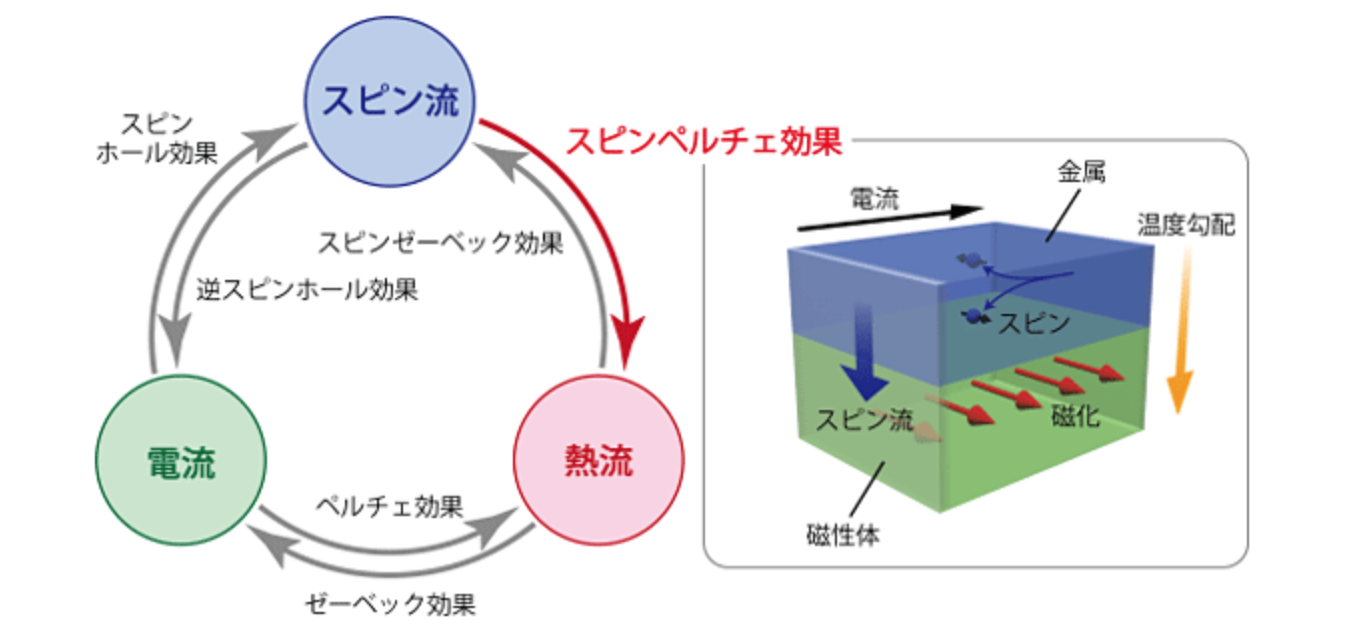
\includegraphics[width=8cm]{./screenshot1.png}
    \caption{スピン流-熱流-電流変換現象とスピンペルチェ効果}
  \end{center}
\end{figure}

\subsection{実験手順}
スピンペルチェの効果を測定するために、金属薄膜(白金もしくはタングステン)と磁気ガーネットの接合構造を用いた。金属薄膜に電流を流すと、金属薄膜と磁気ガーネットの接合界面にスピンホール効果によってスピン流が誘起される。スピンペルチェ効果が生じると、磁性ガーネットの界面を流れるスピンの方向に依存して、加熱もしくは冷却が生じる。今回、この時生じる温度変化を、サーモグラフィ法を応用して熱画像として観測した。\\
スピンペルチェ効果を観測するためには、金属薄膜中を流れる電流に由来するジュール熱による温度変化と、界面を流れるスピン流に由来する温度変化とを分離する必要がある。通常のサーモグラフィ法では、これら2つの温度変化の重ね合わせを測定してしまうため、スピンペルチェ効果による温度変化のみを純粋に測定することは不可能であると考えられてきた。この問題を解決するために、本研究では、ロックイン・サーモグラフィ法と呼ばれる計測技術を利用した。ロックイン・サーモグラフィ法とは、赤外線カメラを用いて、ある周波数で時間変化する温度分布だけを選択的に抽出して可視化する手法。金属薄膜に流れる電流の向きである周波数で切り替えると、ジュール熱は電流の向きによらず一定になるが、スピンペルチェ効果に由来する温度変化は電流の向きに依存して変化する。そのため、ロックイン・サーモグラフィ法によって金属薄膜中の電流と同じ周波数を持つ温度変化信号を検出することで、スピンペルチェ効果に由来する温度分布だけを観測することが可能になる。
\begin{figure}[h]
  \begin{center}
    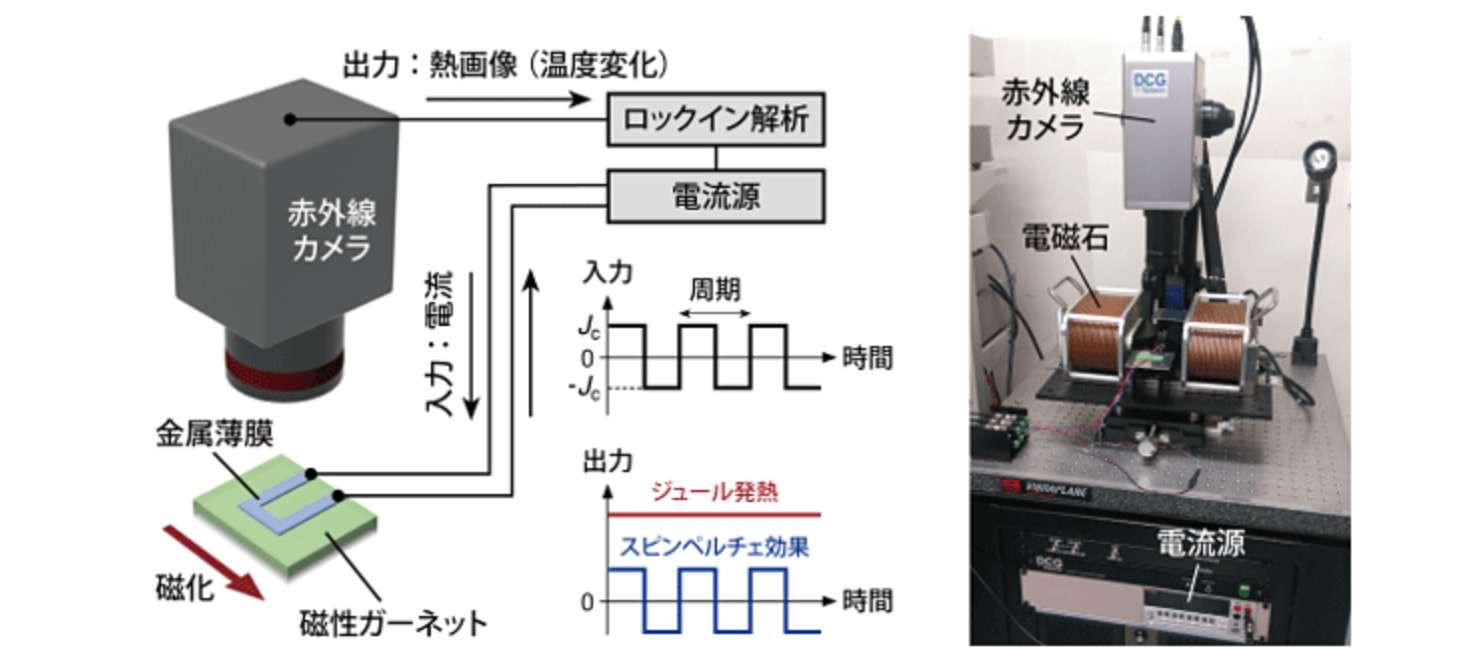
\includegraphics[width=8cm]{./screenshot2.png}
    \caption{ロックイン・サーモグラフィ法によるスピンペルチェ効果計測の概念図と実際の実験系}
  \end{center}
\end{figure}



\subsection{結果}
金属と磁性ガーネットの接合界面上に明瞭な温度変化が観測された。温度変化は電流と磁気の向きが直行している領域にのみ現れていて、電流の向きに依存して温度変化の富豪が反転していることが示された。これらの結果は、電流が生成するスピンの向きに依存した温度変化が生じていることを表しており、観測された現象がスピン流に由来していることを決定づけるものである。本成果により、スピンペルチェ効果の可視化技術を確立することに成功し、スピン流ー熱流変換現象の基礎化学や、それを用いた新たな応用技術を開拓するための基盤が整った。

\begin{figure}[h]
  \begin{center}
    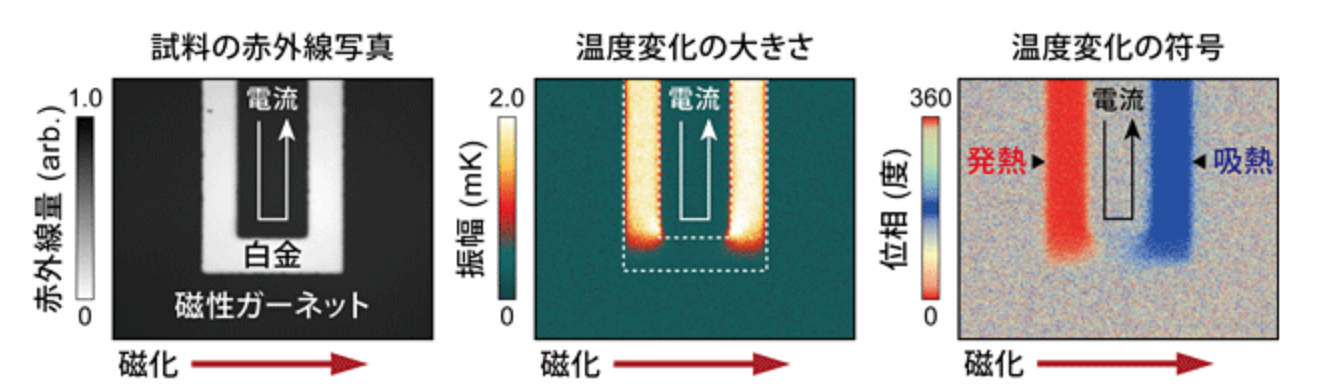
\includegraphics[width=8cm]{./screenshot3.png}
    \caption{白金と磁性ガーネットの接合試料におけるスピンペルチェ効果の熱画像計測}
  \end{center}
\end{figure}

\end{document}
